\documentclass{standalone}
\usepackage{tikz}
\usetikzlibrary{patterns, positioning}
\usepackage[sfdefault]{ClearSans} %% option 'sfdefault' activates Clear Sans as the default text font
\usepackage[T1]{fontenc}

\begin{document}
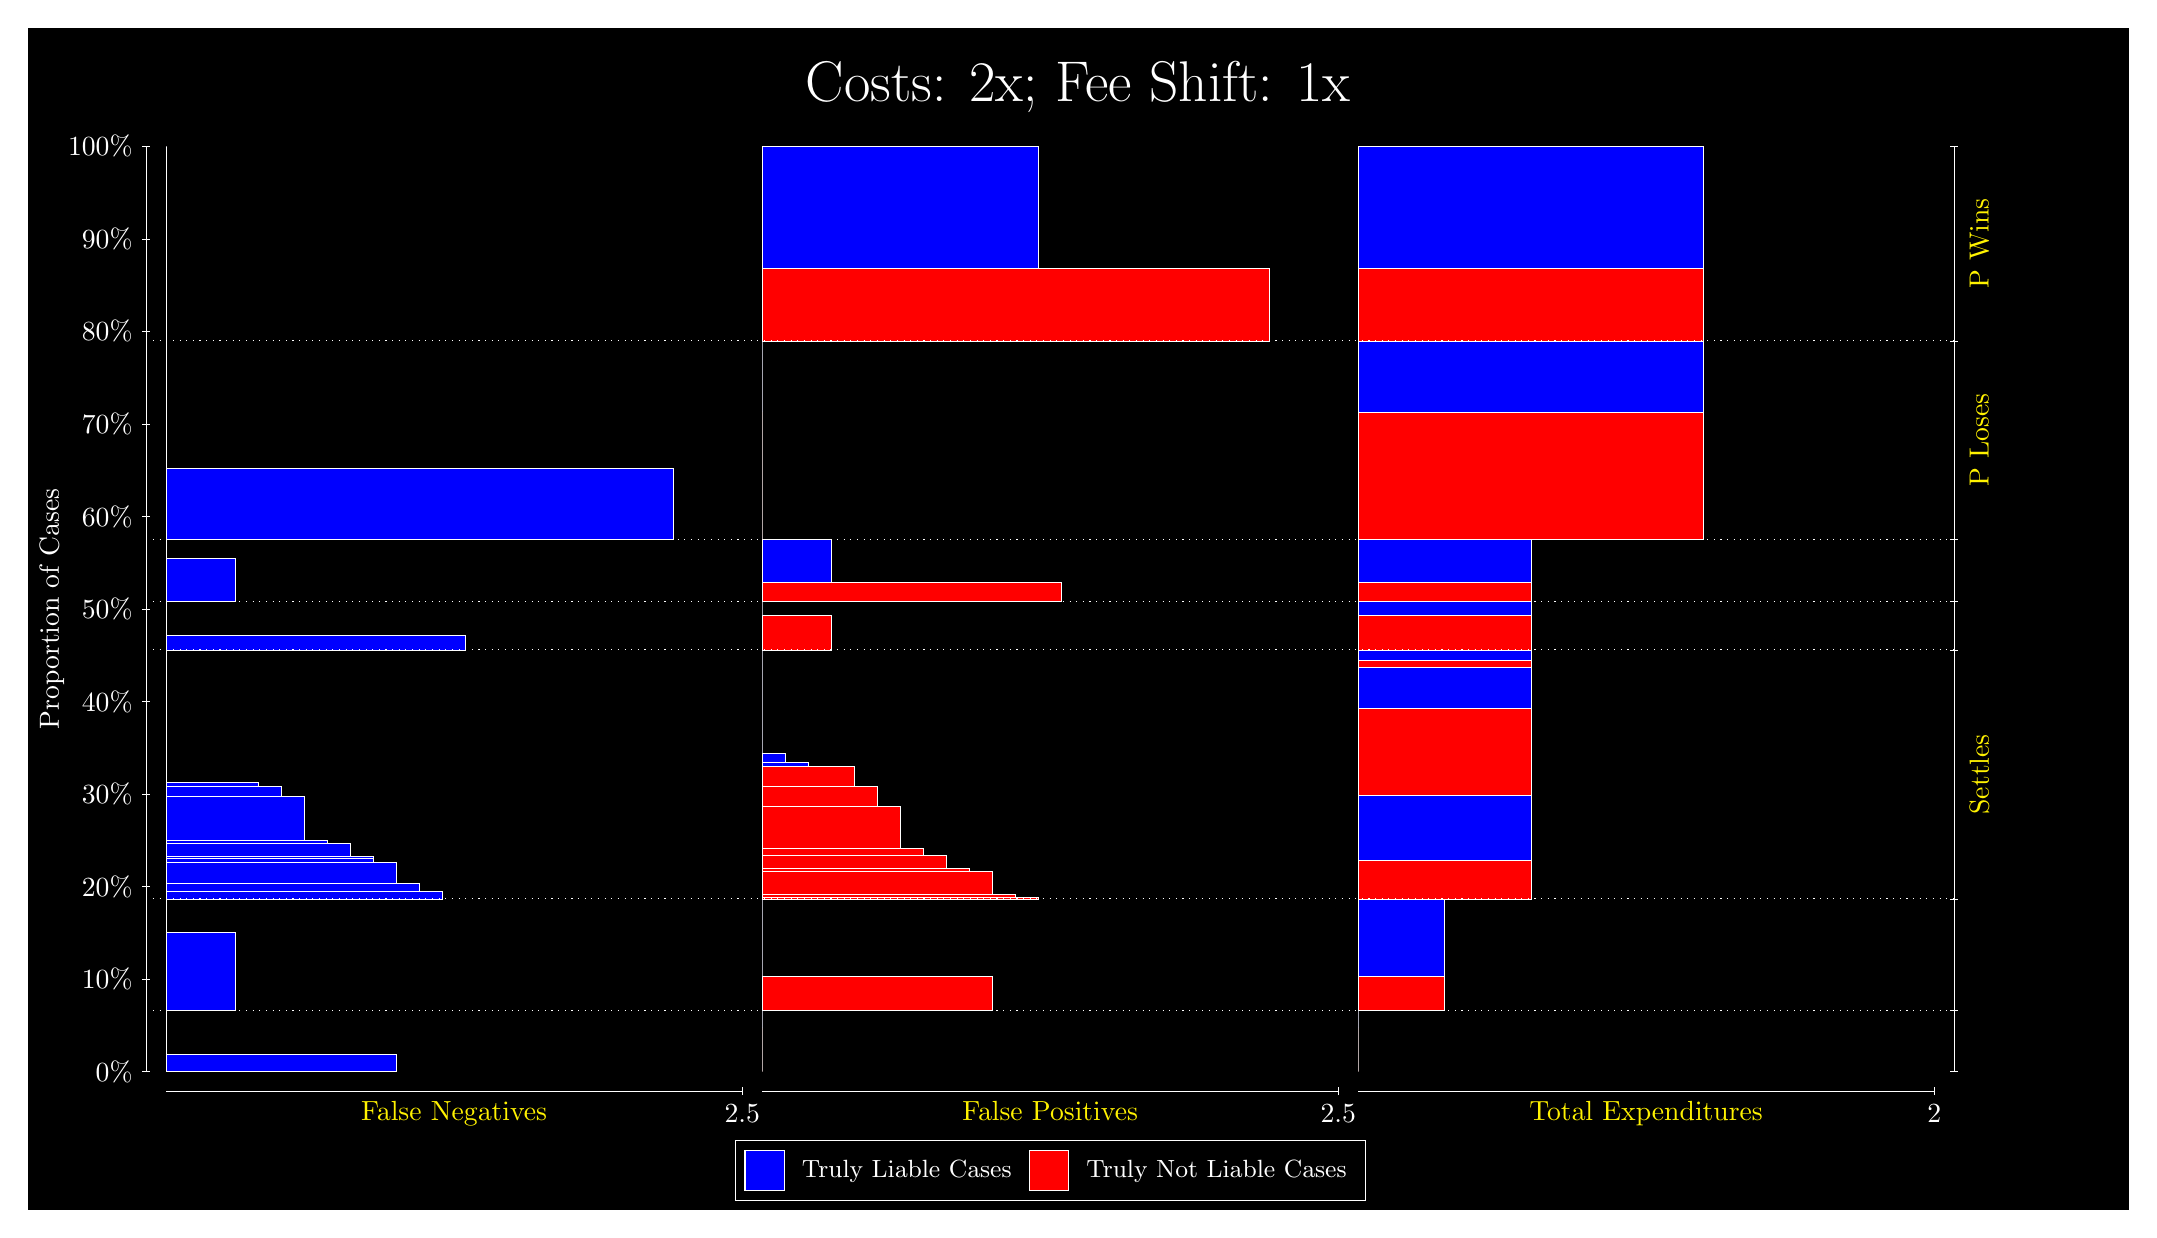
\begin{tikzpicture}
\draw[fill=black] (0,0) rectangle (26.667,15);
\draw[text=white] (0,13.5) rectangle (26.667,15) node[midway] {\huge Costs: 2x; Fee Shift: 1x};
\draw[white, very thin] (1.5,1.75) -- (1.5,13.5);
\node[rotate=90, text=white, anchor=center] at (0.3, 7.625) {Proportion of Cases};
\draw[white, very thin] (1.45,1.75) -- (1.55,1.75);
\node[text=white, anchor=east] at (1.45, 1.75) {0\%};
\draw[white, very thin] (1.45,2.925) -- (1.55,2.925);
\node[text=white, anchor=east] at (1.45, 2.925) {10\%};
\draw[white, very thin] (1.45,4.1) -- (1.55,4.1);
\node[text=white, anchor=east] at (1.45, 4.1) {20\%};
\draw[white, very thin] (1.45,5.275) -- (1.55,5.275);
\node[text=white, anchor=east] at (1.45, 5.275) {30\%};
\draw[white, very thin] (1.45,6.45) -- (1.55,6.45);
\node[text=white, anchor=east] at (1.45, 6.45) {40\%};
\draw[white, very thin] (1.45,7.625) -- (1.55,7.625);
\node[text=white, anchor=east] at (1.45, 7.625) {50\%};
\draw[white, very thin] (1.45,8.8) -- (1.55,8.8);
\node[text=white, anchor=east] at (1.45, 8.8) {60\%};
\draw[white, very thin] (1.45,9.975) -- (1.55,9.975);
\node[text=white, anchor=east] at (1.45, 9.975) {70\%};
\draw[white, very thin] (1.45,11.15) -- (1.55,11.15);
\node[text=white, anchor=east] at (1.45, 11.15) {80\%};
\draw[white, very thin] (1.45,12.325) -- (1.55,12.325);
\node[text=white, anchor=east] at (1.45, 12.325) {90\%};
\draw[white, very thin] (1.45,13.5) -- (1.55,13.5);
\node[text=white, anchor=east] at (1.45, 13.5) {100\%};

\draw[white, very thin] (24.457,1.75) -- (24.457,13.5);
\draw[white, very thin] (24.407,1.75) -- (24.507,1.75);
\node[anchor=west] at (24.407, 1.75) {};
\draw[white, very thin] (24.407,2.5298) -- (24.507,2.5298);
\node[anchor=west] at (24.407, 2.5298) {};
\draw[white, very thin] (24.407,3.9418) -- (24.507,3.9418);
\node[anchor=west] at (24.407, 3.9418) {};
\draw[white, very thin] (24.407,7.1059) -- (24.507,7.1059);
\node[anchor=west] at (24.407, 7.1059) {};
\draw[white, very thin] (24.407,7.7241) -- (24.507,7.7241);
\node[anchor=west] at (24.407, 7.7241) {};
\draw[white, very thin] (24.407,8.5076) -- (24.507,8.5076);
\node[anchor=west] at (24.407, 8.5076) {};
\draw[white, very thin] (24.407,11.029) -- (24.507,11.029);
\node[anchor=west] at (24.407, 11.029) {};
\draw[white, very thin] (24.407,13.5) -- (24.507,13.5);
\node[anchor=west] at (24.407, 13.5) {};

\draw[white, very thin, fill=blue] (1.75,1.75) rectangle (4.6775,1.9748);
\draw[white, very thin, fill=red] (1.75,1.9748) rectangle (1.75,2.5298);
\draw[white, very thin, fill=blue] (1.75,2.5298) rectangle (2.6283,3.5167);
\draw[white, very thin, fill=red] (1.75,3.5167) rectangle (1.75,3.9418);
\draw[white, very thin, fill=blue] (1.75,3.9418) rectangle (5.2631,4.0349);
\draw[white, very thin, fill=blue] (1.75,4.0349) rectangle (4.9703,4.1416);
\draw[white, very thin, fill=blue] (1.75,4.1416) rectangle (4.6775,4.4022);
\draw[white, very thin, fill=blue] (1.75,4.4022) rectangle (4.3848,4.4596);
\draw[white, very thin, fill=blue] (1.75,4.4596) rectangle (4.3848,4.4892);
\draw[white, very thin, fill=blue] (1.75,4.4892) rectangle (4.092,4.6434);
\draw[white, very thin, fill=blue] (1.75,4.6434) rectangle (3.7993,4.6909);
\draw[white, very thin, fill=blue] (1.75,4.6909) rectangle (3.5065,5.2519);
\draw[white, very thin, fill=blue] (1.75,5.2519) rectangle (3.2138,5.3675);
\draw[white, very thin, fill=blue] (1.75,5.3675) rectangle (2.921,5.4259);
\draw[white, very thin, fill=red] (1.75,5.4259) rectangle (1.75,7.1059);
\draw[white, very thin, fill=blue] (1.75,7.1059) rectangle (5.5558,7.2909);
\draw[white, very thin, fill=red] (1.75,7.2909) rectangle (1.75,7.7241);
\draw[white, very thin, fill=blue] (1.75,7.7241) rectangle (2.6283,8.2707);
\draw[white, very thin, fill=red] (1.75,8.2707) rectangle (1.75,8.5076);
\draw[white, very thin, fill=blue] (1.75,8.5076) rectangle (8.1906,9.4092);
\draw[white, very thin, fill=red] (1.75,9.4092) rectangle (1.75,11.029);
\draw[white, very thin, fill=red] (1.75,11.029) rectangle (1.75,11.954);
\draw[white, very thin, fill=blue] (1.75,11.954) rectangle (1.75,13.5);
\draw[white, very thin, fill=red] (9.3189,1.75) rectangle (9.3189,2.305);
\draw[white, very thin, fill=blue] (9.3189,2.305) rectangle (9.3189,2.5298);
\draw[white, very thin, fill=red] (9.3189,2.5298) rectangle (12.246,2.9549);
\draw[white, very thin, fill=blue] (9.3189,2.9549) rectangle (9.3189,3.9418);
\draw[white, very thin, fill=red] (9.3189,3.9418) rectangle (12.832,3.9616);
\draw[white, very thin, fill=red] (9.3189,3.9616) rectangle (12.539,4.0069);
\draw[white, very thin, fill=red] (9.3189,4.0069) rectangle (12.246,4.2873);
\draw[white, very thin, fill=red] (9.3189,4.2873) rectangle (11.954,4.3343);
\draw[white, very thin, fill=red] (9.3189,4.3343) rectangle (11.661,4.4951);
\draw[white, very thin, fill=red] (9.3189,4.4951) rectangle (11.368,4.591);
\draw[white, very thin, fill=red] (9.3189,4.591) rectangle (11.075,5.1151);
\draw[white, very thin, fill=red] (9.3189,5.1151) rectangle (10.783,5.3734);
\draw[white, very thin, fill=red] (9.3189,5.3734) rectangle (10.49,5.6219);
\draw[white, very thin, fill=blue] (9.3189,5.6219) rectangle (9.9044,5.6802);
\draw[white, very thin, fill=blue] (9.3189,5.6802) rectangle (9.6116,5.7959);
\draw[white, very thin, fill=blue] (9.3189,5.7959) rectangle (9.3189,7.1059);
\draw[white, very thin, fill=red] (9.3189,7.1059) rectangle (10.197,7.5391);
\draw[white, very thin, fill=blue] (9.3189,7.5391) rectangle (9.3189,7.7241);
\draw[white, very thin, fill=red] (9.3189,7.7241) rectangle (13.125,7.961);
\draw[white, very thin, fill=blue] (9.3189,7.961) rectangle (10.197,8.5076);
\draw[white, very thin, fill=red] (9.3189,8.5076) rectangle (9.3189,10.127);
\draw[white, very thin, fill=blue] (9.3189,10.127) rectangle (9.3189,11.029);
\draw[white, very thin, fill=red] (9.3189,11.029) rectangle (15.759,11.954);
\draw[white, very thin, fill=blue] (9.3189,11.954) rectangle (12.832,13.5);
\draw[white, very thin, fill=red] (16.888,1.75) rectangle (16.888,2.305);
\draw[white, very thin, fill=blue] (16.888,2.305) rectangle (16.888,2.5298);
\draw[white, very thin, fill=red] (16.888,2.5298) rectangle (17.986,2.9549);
\draw[white, very thin, fill=blue] (16.888,2.9549) rectangle (17.986,3.9418);
\draw[white, very thin, fill=red] (16.888,3.9418) rectangle (19.083,4.4283);
\draw[white, very thin, fill=blue] (16.888,4.4283) rectangle (19.083,5.2591);
\draw[white, very thin, fill=red] (16.888,5.2591) rectangle (19.083,6.3619);
\draw[white, very thin, fill=blue] (16.888,6.3619) rectangle (19.083,6.8797);
\draw[white, very thin, fill=red] (16.888,6.8797) rectangle (19.083,6.9705);
\draw[white, very thin, fill=blue] (16.888,6.9705) rectangle (19.083,7.1059);
\draw[white, very thin, fill=red] (16.888,7.1059) rectangle (19.083,7.5391);
\draw[white, very thin, fill=blue] (16.888,7.5391) rectangle (19.083,7.7241);
\draw[white, very thin, fill=red] (16.888,7.7241) rectangle (19.083,7.961);
\draw[white, very thin, fill=blue] (16.888,7.961) rectangle (19.083,8.5076);
\draw[white, very thin, fill=red] (16.888,8.5076) rectangle (21.279,10.127);
\draw[white, very thin, fill=blue] (16.888,10.127) rectangle (21.279,11.029);
\draw[white, very thin, fill=red] (16.888,11.029) rectangle (21.279,11.954);
\draw[white, very thin, fill=blue] (16.888,11.954) rectangle (21.279,13.5);
\draw[white, dotted] (1.5,2.5298) -- (24.457,2.5298);
\draw[white, dotted] (1.5,3.9418) -- (24.457,3.9418);
\draw[white, dotted] (1.5,7.1059) -- (24.457,7.1059);
\draw[white, dotted] (1.5,7.7241) -- (24.457,7.7241);
\draw[white, dotted] (1.5,8.5076) -- (24.457,8.5076);
\draw[white, dotted] (1.5,11.029) -- (24.457,11.029);
\draw[white, very thin] (1.75,1.5) -- (9.0689,1.5);
\node[text=yellow, anchor=north] at (5.4094, 1.5) {False Negatives};
\draw[white, very thin] (9.0689,1.45) -- (9.0689,1.55);
\node[text=white, anchor=north] at (9.0689, 1.45) {2.5};

\draw[white, very thin] (9.3189,1.5) -- (16.638,1.5);
\node[text=yellow, anchor=north] at (12.978, 1.5) {False Positives};
\draw[white, very thin] (16.638,1.45) -- (16.638,1.55);
\node[text=white, anchor=north] at (16.638, 1.45) {2.5};

\draw[white, very thin] (16.888,1.5) -- (24.207,1.5);
\node[text=yellow, anchor=north] at (20.547, 1.5) {Total Expenditures};
\draw[white, very thin] (24.207,1.45) -- (24.207,1.55);
\node[text=white, anchor=north] at (24.207, 1.45) {2};



\node[text=yellow, centered, rotate=90] at (24.777, 5.5239) {Settles};


\node[text=yellow, centered, rotate=90] at (24.777, 9.7681) {P Loses};
\node[text=yellow, centered, rotate=90] at (24.777, 12.264) {P Wins};

\draw (12.978300999999998,1.5) node[draw=none] (baseCoordinate) {};
\begin{scope}[align=center]
        \matrix[scale=0.5, draw=white, below=0.5cm of baseCoordinate, nodes={draw}, column sep=0.1cm]{
            \node[rectangle, draw, minimum width=0.5cm, minimum height=0.5cm, fill=blue] {}; &
            \node[draw=none, font=\small, text=white] (B) {Truly Liable Cases}; &
            \node[rectangle, draw, minimum width=0.5cm, minimum height=0.5cm, fill=red] {}; &
            \node[draw=none, font=\small, text=white] (B) {Truly Not Liable Cases}; \\
            };
\end{scope}

\end{tikzpicture}
\end{document}